\documentclass[a4paper,11pt]{article}
\usepackage[utf8]{inputenc}
\usepackage[french]{babel}
\usepackage{amsmath,xfrac}
\usepackage[osf,sups]{Baskervaldx} % lining figures
\usepackage[bigdelims,cmintegrals,vvarbb,baskervaldx,frenchmath]{newtxmath} % math font
%\usepackage[cal=boondoxo]{mathalfa} % mathcal from STIX, unslanted a bit
%\usepackage{float}
\usepackage{graphicx}
\usepackage{url,hyperref}
\usepackage{color}

\setlength{\parindent}{0em}
\setlength{\parskip}{1em}
%\addtolength{\hoffset}{-3.5em}
%\addtolength{\textwidth}{7em}
%\addtolength{\voffset}{-5em}
%\addtolength{\textheight}{10em}

%\addtolength{\voffset}{-6em}
%\addtolength{\textheight}{12em}

\begin{document}
\thispagestyle{empty}

\begin{center}
	\Large Vibrations d'un système discret
\end{center}

On considère les trois matrices suivantes:
\[
	D_3=\begin{pmatrix}
		-2 & 1 & 0 \\
		1 & -2 & 1 \\
		0 & 1 & -2 \\
	\end{pmatrix}
	\qquad
	N_3=\begin{pmatrix}
		-1 & 1 & 0 \\
		1 & -2 & 1 \\
		0 & 1 & -1 \\
	\end{pmatrix}
	\qquad
	P_3=\begin{pmatrix}
		-2 & 1 & 1 \\
		1 & -2 & 1 \\
		1 & 1 & -2 \\
	\end{pmatrix}
\]

{\bf Exercice 1.}
Calculez explicitement (à la main) les valeurs et vecteurs propres des
matrices~$X_3$, pour~$X=D,N,P$.

{\sl Indication: les vecteurs propres sont des évaluations des fonctions
trigonométriques sur des positions régulièrement espacées.}

{\bf Exercice 2.}
Définissez des matrices tridiagonales~$D_n$, $N_n$ et $P_n$, de taille~$n\times
n$ pour~$n\ge 3$, qui généralisent le cas particulier~$n=3$.

{\bf Exercice 3.}
À la vue de l'exercice~$1$, trouvez les valeurs et vecteurs propres des
matrices~$D_n$, ~$N_n$ et~$P_n$ pour~$n\ge 3$.

{\bf Définition.}
Si~$A$ est une matrice positive, on dénote par~$\lambda_k(A)$, $k=1,2,\ldots$
les valeurs propres strictement positives de~$A$, ordonnées par ordre croissant.

{\bf Exercice 4.}
Vérifiez que les matrices~$-D_n$, $-N_n$ et $-P_n$ sont positives et donnez une
expression fermée pour les~\emph{partiels}
\[
	\mu_k(X_n) := \sqrt{\frac{\lambda_k(-X_n)}{\lambda_1(-X_n)}}
\]
pour~$X=D,N,P$ et~$k\ge 1$.  Démontrez que quand~$n>>k$ on a~$\mu_k\approx k$,
et estimez la qualité de cette approximation (selon la valeur de~$\tfrac kn$).

{\bf Exercice 5.}
Donnez une interprétation physique à ces matrices et à leurs vecteurs propres.

{\bf Exercice 6.}
Donnez une version continue de toutes ces constructions.

\clearpage
{\bf\large solutions}


{\color{blue}
{\bf Exercice 1.}
Calculez explicitement (à la main) les valeurs et vecteurs propres des
matrices~$X_3$, pour~$X=D,N,P$.
}

On s'intéresse plutôt aux matrices~$-X_n$ car il se trouve qu'elles sont
positives.

\fbox{$D_3$}

%Calculons d'abord les valeurs propres de~$-D_3$, qui sont les racines du
%polynôme caractéristique:
%\[
%	\det\left(\lambda I-D_3\right)
%	=
%	\begin{pmatrix}
%		\lambda-2 & 1 & 0 \\
%		1 & \lambda-2 & 1 \\
%		0 & 1 & \lambda-2 \\
%	\end{pmatrix}
%	=
%	(\lambda-1)^3-2(\lambda-2)
%	=(\lambda - 2)(\lambda^2-4\lambda+2)
%\]
%et les racines sont donc, par ordre croissant
%\[
%	\lambda_1 = 2-\sqrt2
%	\qquad
%	\lambda_2 = 2
%	\qquad
%	\lambda_3 = 2+\sqrt2
%\]
Les vecteurs propres %~$\varphi_1,\varphi_2,\varphi_3$
sont déterminés à un
facteur multiplicatif près.  Par symétrie (la matrice~$D_3$ est invariante par
conjugation
avec~$P=\left(\begin{smallmatrix}0&0&1\\0&1&0\\1&0&0\end{smallmatrix}\right)$),
les vecteurs propres sont symétriques ou anti-symétriques, donc de la
forme~$u=(1,0,-1)$ ou bien~$v_\alpha=(1,\alpha,1)$.  On vérifie que~$D_3u=-2u$,
donc~$u$ est un vecteur propre de~$-D_3$ de valeur propre~$2$.   D'autre côté,
on a~$D_3
v_\alpha
%\left(\begin{smallmatrix}1\\\alpha\\1\end{smallmatrix}\right)
=
\left(\begin{smallmatrix}\alpha-2\\2-2\alpha\\\alpha-2\end{smallmatrix}\right)
=
(\alpha-2)
v_\frac{2-2\alpha}{\alpha-2}
%\left(\begin{smallmatrix}1\\\frac{2-2\alpha}{\alpha-2}\\1\end{smallmatrix}\right)
$.  Si~$v_\alpha$ est un vecteur propre il faudra donc
que~$\alpha=\frac{2-2\alpha}{\alpha-2}$, ou équivalemment~$\alpha=\pm\sqrt 2$
et les valeurs propres associées sont~$2\pm\sqrt 2$.
Ainsi, les trois valeurs
propres de~$-D_3$ sont, par ordre croissant
\[
	\lambda_1 = 2-\sqrt2
	\qquad
	\lambda_2 = 2
	\qquad
	\lambda_3 = 2+\sqrt2
\]
et les vecteurs propres correspondants, normalisés avec la norme sup:
\[
	\varphi_1=\begin{pmatrix}
		\sfrac{\sqrt2}2\\
		1\\
		\sfrac{\sqrt2}2
	\end{pmatrix}
	\qquad
	\varphi_2=\begin{pmatrix}
		1\\
		0\\
		-1
	\end{pmatrix}
	\qquad
	\varphi_3=\begin{pmatrix}
		\sfrac{\sqrt2}2\\
		-1\\
		\sfrac{\sqrt2}2
	\end{pmatrix}
\]
Observez que les vecteurs propres sont des évaluations de~$\sin\tfrac\theta2$
sur 4 points equi-espacés~$\varphi_n^k=\sin\frac{nk\pi}2,\ k,\!n=1,2,3$.

%SCRIPT cat <<END | gnuplot > f/sind3.pdf
%%SCRIPT set term pngcairo crop size 800,400
%SCRIPT set term pdfcairo crop size 5,2.5
%SCRIPT set samples 1000
%SCRIPT set key bottom left box opaque
%SCRIPT set xtics (0, "{/Symbol p}/2" 0.5*pi, "{/Symbol p}" pi, "3{/Symbol p}/2" 1.5*pi, "2{/Symbol p} "2*pi)
%SCRIPT set ytics (-1, 0, "1/{/Symbol \326}2" sqrt(2)/2, 1)
%SCRIPT set arrow from pi/2, graph 0 to pi/2, graph 1 nohead dt 2
%SCRIPT set arrow from 3*pi/2, graph 0 to 3*pi/2, graph 1 nohead dt 2
%SCRIPT set arrow from pi, graph 0 to pi, graph 1 nohead dt 2
%SCRIPT set arrow from 0, 0 to 2*pi, 0 nohead dt 2
%SCRIPT set arrow from 0, 0 to 2*pi, 0 nohead dt 2
%SCRIPT set arrow from 0, 1/sqrt(2) to 2*pi, 1/sqrt(2) nohead dt 2
%SCRIPT set arrow from 0, -1 to 2*pi, -1 nohead dt 2
%SCRIPT set arrow from 0, 1 to 2*pi, 1 nohead dt 2
%SCRIPT set obj circle at pi/2,1/sqrt(2) radius .06 fc rgb "red" fs solid
%SCRIPT set obj circle at pi,1 radius .06 fc rgb "red" fs solid
%SCRIPT set obj circle at 3*pi/2,1/sqrt(2) radius .06 fc rgb "red" fs solid
%SCRIPT set obj circle at pi/2,1 radius .06 fc rgb "blue" fs solid
%SCRIPT set obj circle at pi,0 radius .06 fc rgb "blue" fs solid
%SCRIPT set obj circle at 3*pi/2,-1 radius .06 fc rgb "blue" fs solid
%SCRIPT set obj circle at pi/2,1/sqrt(2) radius .06 fc rgb "dark-green" fs solid
%SCRIPT set obj circle at pi,-1 radius .06 fc rgb "dark-green" fs solid
%SCRIPT set obj circle at 3*pi/2,1/sqrt(2) radius .06 fc rgb "dark-green" fs solid
%SCRIPT plot [0:2*pi] [-1.2:1.2] sin(1*x/2) lw 3 lc rgb "red", sin(2*x/2) lw 3 lc rgb "blue", sin(3*x/2) lw 3 lc rgb "dark-green"
%SCRIPT END
\begin{center}
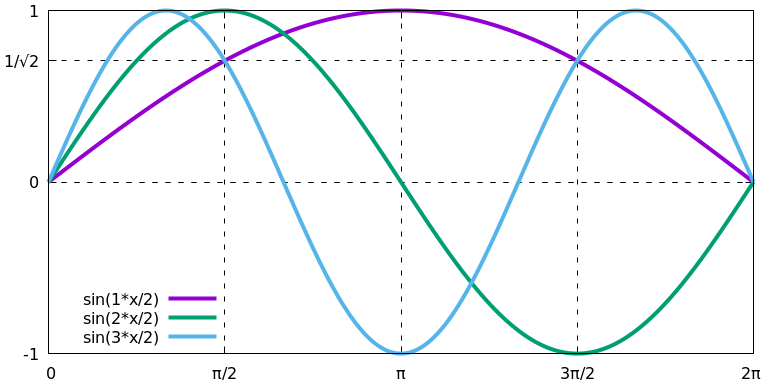
\includegraphics[width=.9\textwidth]{f/sind3.pdf}
\end{center}

\clearpage

\fbox{$N_3$}

Les lignes de la matrice~$N_3$ sont de somme nulle, donc~$(1,1,1)$ est un
vecteur propre de valeur propre nulle.  Par le même argument que sur~$D_3$, les
autres vecteurs propres doivent être symétriques ou anti-symétriques.  On voit
d'abord que~$u=(1,0,-1)$ est un vecteur propre de valeur propre~$1$; et que
si~$v_\alpha(1,\alpha,1)$ est un vecteur propre alors~$N_3v_\alpha=
\left(\begin{smallmatrix}\alpha-1\\2-2\alpha\\\alpha-1\end{smallmatrix}\right)=(\alpha-1)v_{\frac{2-2\alpha}{\alpha-1}}$,
donc si~$v_\alpha$ est un vecteur propre
alors~$\alpha=\frac{2-2\alpha}{\alpha-1}$ ou équivalemment~$\alpha=1,-2$.
Pour~$\alpha=1$ on récupère le vecteur propre~$(1,1,1)$ et pour~$\alpha=-2$ on
trouve un vecteur propre~$(1,-2,1)$ de valeur propre~$3$.
Ainsi, les trois valeurs
propres de~$-N_3$ sont, par ordre croissant
\[
	\lambda_1 = 0
	\qquad
	\lambda_2 = 1
	\qquad
	\lambda_3 = 3
\]
et les vecteurs propres correspondants, normalisés ``de façon naturelle'':
\[
	\varphi_1=\begin{pmatrix}
		1\\
		1\\
		1
	\end{pmatrix}
	\qquad
	\varphi_2=\begin{pmatrix}
		\sfrac{\sqrt3}2\\
		0\\
		-\sfrac{\sqrt3}2
	\end{pmatrix}
	\qquad
	\varphi_3=\begin{pmatrix}
		\sfrac12\\
		-1\\
		\sfrac12\\
	\end{pmatrix}
\]
Observez que les vecteurs propres sont des évaluations de~$\cos\tfrac\theta2$
sur 3 points equi-espacés~$\varphi_n^k=\cos\frac{(n-1)k?\pi}3,\ k,\!n=1,2,3$.

%SCRIPT cat <<END | gnuplot > f/cosn3.pdf
%SCRIPT set term pdfcairo size 5,2.5
%SCRIPT set samples 1000
%SCRIPT set key bottom left box opaque
%SCRIPT set xtics (0, "{/Symbol p}/3" pi/3, "{/Symbol p}" pi, "5{/Symbol p}/3" 5*pi/3, "2{/Symbol p} "2*pi)
%SCRIPT set ytics (-1, "{/Symbol \326}3/2" -sqrt(3)/2, 0, "1/2" 0.5, "{/Symbol \326}3/2" sqrt(3)/2, 1)
%SCRIPT set arrow from pi/3, graph 0 to pi/3, graph 1 nohead dt 2
%SCRIPT set arrow from 5*pi/3, graph 0 to 5*pi/3, graph 1 nohead dt 2
%SCRIPT set arrow from pi, graph 0 to pi, graph 1 nohead dt 2
%SCRIPT set arrow from 0, 0 to 2*pi, 0 nohead dt 2
%SCRIPT set arrow from 0, 0 to 2*pi, 0 nohead dt 2
%SCRIPT set arrow from 0, 0.5 to 2*pi, 0.5 nohead dt 2
%SCRIPT set arrow from 0, sqrt(3)/2 to 2*pi, sqrt(3)/2 nohead dt 2
%SCRIPT set arrow from 0, -sqrt(3)/2 to 2*pi, -sqrt(3)/2 nohead dt 2
%SCRIPT set arrow from 0, -1 to 2*pi, -1 nohead dt 2
%SCRIPT set obj circle at pi/3,1 radius .06 fc rgb "red" fs solid
%SCRIPT set obj circle at pi,1 radius .06 fc rgb "red" fs solid
%SCRIPT set obj circle at 5*pi/3,1 radius .06 fc rgb "red" fs solid
%SCRIPT set obj circle at pi/3,sqrt(3)/2 radius .06 fc rgb "blue" fs solid
%SCRIPT set obj circle at pi,0 radius .06 fc rgb "blue" fs solid
%SCRIPT set obj circle at 5*pi/3,-sqrt(3)/2 radius .06 fc rgb "blue" fs solid
%SCRIPT set obj circle at pi/3,.5 radius .06 fc rgb "dark-green" fs solid
%SCRIPT set obj circle at pi,-1 radius .06 fc rgb "dark-green" fs solid
%SCRIPT set obj circle at 5*pi/3,.5 radius .06 fc rgb "dark-green" fs solid
%SCRIPT plot [0:2*pi] [-1.2:1.2] cos(0*x/2) lw 3 lc rgb "red", cos(1*x/2) lw 3 lc rgb "blue", cos(2*x/2) lw 3 lc rgb "dark-green"
%SCRIPT END
\begin{center}
\includegraphics[width=.9\textwidth]{f/cosn3.pdf}

\end{center}

\clearpage

\fbox{$P_3$}

Le calcul pour~$-P_3$ est différent puisqu'il y a des valeurs propres répétés:
\[
	\det\left(\lambda I + P_3\right)
	=
	\left|
	\begin{matrix}
		\lambda-2 & 1 & 1 \\
		1 & \lambda-2 & 1 \\
		1 & 1 & \lambda-2 \\
	\end{matrix}
	\right|
	=\lambda(\lambda-3)^2
\]
On a alors un vecteur propre~$(1,1,1)$ de valeur propre~$0$, et un sous-espace
propre de dimension~$2$, associé au valeur propre~$3$.  Par commodité, on peut
choisir une base orthogonale de cet sous-espace constituée par un vecteur
symétrique et un vecteur anti-symétrique.  Ainsi, on obtient les mêmes vecteurs
propres que pour~$N_3$, mais n'oublions pas que c'est un choix essentiellement
arbitraire.  Les valeurs propres sont:
\[
	\lambda_1 = 0
	\qquad
	\lambda_2 = 3
	\qquad
	\lambda_3 = 3
\]
et les vecteurs propres correspondants peuvent être choisis ainsi
\[
	\varphi_1=\begin{pmatrix}
		1\\
		1\\
		1
	\end{pmatrix}
	\qquad
	\varphi_2=\begin{pmatrix}
		\sfrac{\sqrt3}2\\
		0\\
		-\sfrac{\sqrt3}2
	\end{pmatrix}
	\qquad
	\varphi_3=\begin{pmatrix}
		\sfrac12\\
		-1\\
		\sfrac12\\
	\end{pmatrix}
\]
À noter que l'on peut appliquer des rotations d'angle arbitraire autour de
l'axe~$(3,2,3)$ sur les vecteurs~$\varphi_2,\varphi_3$ pour obtenir une famille
de bases orthogonales de vecteurs propres.


%SCRIPT cat <<END | gnuplot > f/sincosp3.pdf
%SCRIPT set term pdfcairo crop size 5,2.5
%SCRIPT set samples 1000
%SCRIPT set key bottom left box opaque
%SCRIPT set xtics (0, "{/Symbol p}/3" pi/3, "{/Symbol p}" pi, "5{/Symbol p}/3" 5*pi/3, "2{/Symbol p} "2*pi)
%SCRIPT set ytics (-1, "{/Symbol \326}3/2" -sqrt(3)/2, 0, "1/2" 0.5, "{/Symbol \326}3/2" sqrt(3)/2, 1)
%SCRIPT set arrow from pi/3, graph 0 to pi/3, graph 1 nohead dt 2
%SCRIPT set arrow from 5*pi/3, graph 0 to 5*pi/3, graph 1 nohead dt 2
%SCRIPT set arrow from pi, graph 0 to pi, graph 1 nohead dt 2
%SCRIPT set arrow from 0, 0 to 2*pi, 0 nohead dt 2
%SCRIPT set arrow from 0, 0 to 2*pi, 0 nohead dt 2
%SCRIPT set arrow from 0, 0.5 to 2*pi, 0.5 nohead dt 2
%SCRIPT set arrow from 0, sqrt(3)/2 to 2*pi, sqrt(3)/2 nohead dt 2
%SCRIPT set arrow from 0, -sqrt(3)/2 to 2*pi, -sqrt(3)/2 nohead dt 2
%SCRIPT set arrow from 0, 1 to 2*pi, 1 nohead dt 2
%SCRIPT set arrow from 0, -1 to 2*pi, -1 nohead dt 2
%SCRIPT set obj circle at pi/3,1 radius .06 fc rgb "red" fs solid
%SCRIPT set obj circle at pi,1 radius .06 fc rgb "red" fs solid
%SCRIPT set obj circle at 5*pi/3,1 radius .06 fc rgb "red" fs solid
%SCRIPT set obj circle at pi/3,sqrt(3)/2 radius .06 fc rgb "blue" fs solid
%SCRIPT set obj circle at pi,0 radius .06 fc rgb "blue" fs solid
%SCRIPT set obj circle at 5*pi/3,-sqrt(3)/2 radius .06 fc rgb "blue" fs solid
%SCRIPT set obj circle at pi/3,.5 radius .06 fc rgb "dark-green" fs solid
%SCRIPT set obj circle at pi,-1 radius .06 fc rgb "dark-green" fs solid
%SCRIPT set obj circle at 5*pi/3,.5 radius .06 fc rgb "dark-green" fs solid
%SCRIPT plot [0:2*pi] [-1.2:1.2] cos(0*x) lw 3 lc rgb "red", sin(1*x) lw 3 lc rgb "blue", cos(1*x) lw 3 lc rgb "dark-green"
%SCRIPT END
\begin{center}
\includegraphics[width=.9\textwidth]{f/sincosp3.pdf}
\end{center}


\clearpage

{\color{blue}
{\bf Exercice 2.}
Définissez des matrices tridiagonales~$D_n$, $N_n$ et $P_n$, de taille~$n\times
n$ pour~$n\ge 3$, qui généralisent le cas particulier~$n=3$.

{\color{blue}
{\bf Exercice 3.}
À la vue de l'exercice~$1$, trouvez les valeurs et vecteurs propres des
matrices~$D_n$, ~$N_n$ et~$P_n$ pour~$n\ge 3$.
}

{\color{blue}
{\bf Exercice 4.}
Vérifiez que les matrices~$-D_n$, $-N_n$ et $-P_n$ sont positives et donnez une
expression fermée pour les~\emph{partiels}
\[
	\mu_k(X_n) := \sqrt{\frac{\lambda_k(-X_n)}{\lambda_1(-X_n)}}
\]
pour~$X=D,N,P$ et~$k\ge 1$.  Démontrez que quand~$n>>k$ on a~$\mu_k\approx k$,
et estimez la qualité de cette approximation (selon la valeur de~$\tfrac kn$).
}

{\color{blue}
{\bf Exercice 5.}
Donnez une interprétation physique à ces matrices et à leurs vecteurs propres.
}

{\color{blue}
{\bf Exercice 6.}
Donnez une version continue de toutes ces constructions.
}


\end{document}


% vim:set tw=79 spell spelllang=fr:
